\documentclass[a4paper,11pt]{article}
\usepackage{amsmath,amsthm,amsfonts,amssymb,amscd,amstext,vmargin,graphics,graphicx,tabularx,multicol} 
\usepackage[francais]{babel}
\usepackage[utf8]{inputenc}  
\usepackage[T1]{fontenc} 
\usepackage{pstricks-add,tikz,tkz-tab,variations}
\usepackage[autolanguage,np]{numprint} 
\usepackage{color}

\setmarginsrb{1.5cm}{0.5cm}{1cm}{0.5cm}{0cm}{0cm}{0cm}{0cm} %Gauche, haut, droite, haut
\newcounter{numexo}
\newcommand{\exo}[1]{\stepcounter{numexo}\noindent{\bf Exercice~\thenumexo} : \marginpar{\hfill /#1}}
\reversemarginpar


\newcounter{enumtabi}
\newcounter{enumtaba}
\newcommand{\q}{\stepcounter{enumtabi} \theenumtabi.  }
\newcommand{\qa}{\stepcounter{enumtaba} (\alph{enumtaba}) }
\newcommand{\initq}{\setcounter{enumtabi}{0}}
\newcommand{\initqa}{\setcounter{enumtaba}{0}}

\newcommand{\be}{\begin{enumerate}}
\newcommand{\ee}{\end{enumerate}}
\newcommand{\bi}{\begin{itemize}}
\newcommand{\ei}{\end{itemize}}
\newcommand{\bp}{\begin{pspicture*}}
\newcommand{\ep}{\end{pspicture*}}
\newcommand{\bt}{\begin{tabular}}
\newcommand{\et}{\end{tabular}}
\renewcommand{\tabularxcolumn}[1]{>{\centering}m{#1}} %(colonne m{} centrée, au lieu de p par défault) 
\newcommand{\tnl}{\tabularnewline}

\newcommand{\bmul}[1]{\begin{multicols}{#1}}
\newcommand{\emul}{\end{multicols}}

\newcommand{\trait}{\noindent \rule{\linewidth}{0.2mm}}
\newcommand{\hs}[1]{\hspace{#1}}
\newcommand{\vs}[1]{\vspace{#1}}

\newcommand{\N}{\mathbb{N}}
\newcommand{\Z}{\mathbb{Z}}
\newcommand{\R}{\mathbb{R}}
\newcommand{\C}{\mathbb{C}}
\newcommand{\Dcal}{\mathcal{D}}
\newcommand{\Ccal}{\mathcal{C}}
\newcommand{\mc}{\mathcal}

\newcommand{\vect}[1]{\overrightarrow{#1}}
\newcommand{\ds}{\displaystyle}
\newcommand{\eq}{\quad \Leftrightarrow \quad}
\newcommand{\vecti}{\vec{\imath}}
\newcommand{\vectj}{\vec{\jmath}}
\newcommand{\Oij}{(O;\vec{\imath}, \vec{\jmath})}
\newcommand{\OIJ}{(O;I,J)}


\newcommand{\reponse}[1][1]{%
\multido{}{#1}{\makebox[\linewidth]{\rule[0pt]{0pt}{20pt}\dotfill}
}}

\newcommand{\titre}[5] 
% #1: titre #2: haut gauche #3: bas gauche #4: haut droite #5: bas droite
{
\noindent #2 \hfill #4 \\
#3 \hfill #5

\vspace{-1.6cm}

\begin{center}\rule{6cm}{0.5mm}\end{center}
\vspace{0.2cm}
\begin{center}{\large{\textbf{#1}}}\end{center}
\begin{center}\rule{6cm}{0.5mm}\end{center}
}



\begin{document}
\pagestyle{empty}
\titre{Contrôle sur le théorème de Thalès }{Nom :}{Prénom :}{Classe}{Date}


\vspace*{0.5cm}

\exo{2} Placer les points manquants sur la figure sachant que :\\
\hspace*{2cm}- les droites $(d_{1})$ et $(d_{2})$ sont parallèles \\
\hspace*{2cm}- $\dfrac{AB}{AL}=\dfrac{AC}{AM}=\dfrac{BC}{LM}$ 

\begin{center}
\includegraphics[scale=0.7]{thalescours.eps} 
\end{center}



\vspace*{0.5cm}

\exo{7} Soit EFG un triangle tel que EF = 5 cm ; EG = 4 cm et FG = 3,3 cm.  \\
On appelle M, le point de [EG) tel que EM = 6 cm. \\
La parallèle à (FG) passant par le point M coupe [EF) en N. \\

\initq \q Construire cette figure en grandeur réelle sur votre copie.\\

\q Calculer les longueurs EN et MN. (Justifier rigoureusement votre réponse en utilisant le théorème de Thalès) 

\vspace*{1cm}

\exo{5} Un homme mesurant 1,75 m se tenant droit aux alentours de la tour Eiffel se place de sorte que l'ombre lui passe juste au dessus de la tête. \\
Son ombre tombe à 2,7 m de lui et celle-ci
se trouve à 500 m du centre de la tour Eiffel.\\
On supposera pour cet exercice que la tour Eiffel est bien parallèle à l'homme qui se tient debout.\\


\begin{center}
\includegraphics[scale=0.7]{thalestouraiffel.eps} 

\end{center}
\textbf{Quel est la hauteur de la tour Eiffel? (arrondie au mètre près)}\\

\newpage
\vspace*{1cm}

\exo{6}

\noindent Dans les marais salants, le sel récolté est stocké sur une surface plane.
On admet qu'un tas de sel a toujours la forme d'un cône de révolution.\\
Pascal souhaite déterminer la hauteur d'un cône de sel de diamètre 5 mètres. Il possède un bâton de longueur 1 mètre. Il effectue des mesures et réalise les deux schémas ci-dessous.\\



\includegraphics[scale=1]{thales2.eps} 



\vspace*{0.5cm}



\textbf{Démontrer que la hauteur de ce cône de sel est égale à 2,5 mètres.} (\textit{Pensez à justifier que les droites (SO) et (CB) sont bien parallèles.) }\\


\vspace*{0.5cm}


\end{document}
